\section{Phase 2: Planung und Durchführung der Datenerhebung}
\label{sec:datenerhebung}\label{sec:phase2}

Da nun die gröbsten Usability-Probleme --- insbesondere bzgl. der Out-Of-Of-Experience --- beseitigt wurden, kann mit der Erforschung der API im engeren Sinne fortgefahren werden. Dazu habe ich für die Analyse, der in diesem Abschnitt vorgestellten erhobenen Daten, die \gls{gtm} verwendet, welche ich bereits im \sref{sec:gtm} vorgestellt habe.

Um eine für die Analysezwecke sinnvolle Datenerhebung zu planen, lohnt sich zunächst der Vergleich mit anderen Studien.



\subsection{Vergleich mit anderen Studien}

In der Arbeit von \cite{deSouza:2004fd} wurde eine nicht-partizipative Feldstudie über einen Zeitraum von 11 Wochen durchgeführt. Dabei wurden Beobachtungen auf nicht weitere definierte Weise festgehalten und semi-strukturierte Interviews durchgeführt.

Bei der fachlich-nahen Arbeit von \cite{Letondal:2006dy} wurden für die Entwicklung eines Anwendung-Entwicklungsumgebung-Hybriden (Ansatz: \textit{Programming In The User Interface}), über mehrere Iterationen hinweg, größtenteils Brainstorming-Sessions und teilweise videoaufgezeichnete Interviews eingesetzt (Details siehe \sref{sec:letondal}).

In der Clarkeschen Forschung \citep[u.a.][]{clarke:2006} werden API-Anwender bei der Lösung gestellter Programmieraufgaben videoaufgezeichnet.

\cite{LaToza:2007fj} beobachtete bei seiner Arbeit ebenfalls Entwickler und zeichnete diese mit Video auf. Des Weiteren wurden die Entwickler instruiert, lautes Denken (engl. \textit{Think Aloud}) anzuwenden. Am außergewöhnlichsten ist jedoch die Instrumentalisierung der \gls{eclipse}-Entwicklungsumgebung, mit deren Hilfe die Autoren diverse Ereignisse innerhalb der Entwicklungsumgebung mitgeschnitten haben. Details zur dieser Arbeit finden sich im \sref{sec:FactFinding}.

Bei der im \sref{sec:concept-maps} näher beschriebenen Concept-Maps-Methode \citep{Tenny:2011jp} werden informelle Gruppendiskussionen mit den API-Entwicklern und -Anwendern geführt und die Ergebnisse an einem Flipchart, für alle zugänglich, festgehalten.

\cite{Grill:2012jm} stellen in ihrer Fallstudie ein Verfahren zur API-Usability-Evaluation vor und nutzen dabei Workshops, die den beim BioStore-Projekt eingesetzten, ähneln. Während dieser Workshops werden API-Anwender bei ihrer Arbeit videoaufgezeichnet und im Anschluss interviewt. Weitere Details finden sich im \sref{sec:grill}.

\cite{Piccioni:2013uq} verwendeten zur Verbesserung einer Persistenz-Bibliothek ebenfalls Videoaufzeichnungen von Problem-lösenden API-Anwendern und anschließenden Interviews (Details siehe \sref{sec:piccioni}).


\subsubsection{Kombination von Methoden}

Die meisten genannten Arbeiten verwenden eine Kombination verschiedener Datenerhebungs- und Analysemethoden. Für die Kombination der, in der klassischen Usability-Evaluation gebräuchlichen Methoden \textit{\acrlong{he}} \citep{Nielsen:1990bw} und \textit{Usability-Test} \citep{Faulkner:2003wn} konnte bereits gezeigt werden, dass diese verschiedenartige Usability-Probleme aufdecken und ideal kombiniert werden können \citep{Fu:2002tp}.

Eine ähnliche Beobachtung konnten \cite{Grill:2012jm} bei der Kombination von semi-strukturierten Interviews und Videoaufzeichnungen machen. Ihre Analyse beider Quellen förderte 168 API-Usablity-Probleme zu Tage, von denen 157 in nur einer der beiden Datenquellen zu finden waren. Sie stellten beispielsweise fest, dass sich Laufzeit-Probleme nicht mit einer \gls{he} auffinden konnten. Außerdem bemerkten sie, dass sie zwar die meisten Probleme mit Hilfe der Interviews fanden, die schwerwiegendsten Probleme jedoch in den Videoaufzeichnungen verborgen waren. Ähnliche Erfahrungen haben auch \cite{Piccioni:2013uq} gemacht.


\subsubsection{Subjektive und objektive Daten}
\label{sec:objektive-vs-subjektive-Daten}

Es gibt in der API-Usability-Forschung einen Trend zur Betonung subjektiver Daten \citep{Rosson:2001uf,Stylos:2008cu,Robillard:2010bh}, dem auch alle mir bekannten API-Evaluationsstudien folgen. Auch wenn Videoaufzeichnungen, technisch betrachtet, objektive Daten darstellen\footnote{\sref{sec:def-usability} befasst sich mit den Klassen der Erhebungs- und Analyseverfahren.}, werden diese meist nur verwendet, um Erklärungslücken bei der Analyse von Interviews zu klären \citep[vgl.][]{Letondal:2006dy,Grill:2012jm,Tenny:2011jp} oder quantitative Betrachtungen vorzunehmen \citep[vgl.][]{Piccioni:2013uq}. Ausschließlich objektive Daten verwenden nach meiner Kenntnis nur zwei API-Evaluationsstudien \citep{deSouza:ek,Watson:2009bm}.

Tatsächlich sind aber beide Datentypen\footnote{Subjektive Verfahren erheben subjektive Meinungen/Ansichten/Darlegungen der Benutzer, wohingegen objektive Verfahren direkt beobachtbare Daten erfassen. Eine ausführlichere Differenzierung beschreiben \cite{Sarodnick:2006vc}.} wichtig:
\begin{description}
  \item[Subjektive Daten] erhalten viele relevante Informationen zu Usability-Problemen \citep{Rosson:2001uf,Stylos:2008cu,Robillard:2010bh,DaqingHou:2005ba}, z.B. in Bezug auf die Anforderungen an das Softwaresystem \citep{eagan2008buzz}. Allerdings besteht die Gefahr, dass Befragte manchen für irrelevant gehaltenen \citep{Daughtry:2009be} oder kritischen Punkt in Interviews \citep[\textit{soziale Erwünschtheit},][]{Hartmann:1991ju} bzw. in Gruppendiskussionen \citep[\textit{Schweigespirale},][]{NoelleNeumann:1989db} nicht äußern. Ebenso so schwer wiegt, dass Probanden auch nur Äußerungen zu Punkten machen können, die ihnen bewusst sind \citep{Ko:2011el}.
  \item[Objektive Daten] In objektiven Daten hingegen manifestieren sich Probleme, die dem Anwender möglicherweise nicht bewusst sind oder nicht korrekt erfragt wurden \citep{Ko:2011el}. Gegebenenfalls kann der Befragte ein Problem nicht verbalisieren, weil er es bereits gelöst hat, bevor er jemals danach gefragt wurde \citep{sunshine2014searching}.
\end{description}

Die Mischung beider Datentypen vereint die jeweiligen Vorteile \citep{Sarodnick:2006vc}. Im Laufe dieser Arbeit habe ich die Erfahrung gemacht, dass die qualitative Analyse objektiver Daten anspruchsvoller ist, als die subjektiver Daten. Objektive Daten enthalten häufig weniger Hinweise darauf, ``wo die Musik spielt''.



\subsubsection{Studienformen}

Die meisten mir bekannten API-Usability relevanten Studien sind Labor- oder Fallstudien. Zu den wenigen partizipativen Feldstudien gehören \cite{Letondal:2006dy} und \cite{Tenny:2011jp}. Die einzige mir bekannte nicht-partizipative Feldstudie ist die von \cite{deSouza:2004fd}.

Langzeitstudien sind rar. Zwei Studien \citep{Tenny:2011jp,deSouza:2004fd} machten Feldbeobachtungen über jeweils elf Wochen hinweg. Die Arbeit von \cite{Letondal:2006dy} fußt auf Datenerhebungen, die über einen Zeitraum von acht Jahren angefertigt wurden.





\subsection{Planung der Datenerhebung}

\subsubsection{Ziele}

Die von mir geplante Datenerhebung, verfolgte zwei primäre Ziele:
\begin{enumerate}
  \item Die Datenerhebung sollte so reichhaltig wie möglich sein, denn die möglichen Zeitpunkte zur Datenerhebung waren begrenzt.
  \item Die Datenerhebung sollte so wenig wie möglich, die Arbeit der SeqAn-API-Anwender beeinflussen, um verallgemeinerbare Aussagen treffen zu können.
\end{enumerate}


\subsubsection{Anforderungen}

Für die Datenerhebung musste ich ein Verfahren entwickeln, das die eben beschriebenen primären Ziele und die daraus folgenden Anforderungen erfüllt:
\begin{itemize}
  \item Die Daten müssen auf den individuellen Arbeitsplätzen der Probanden erhoben werden. Die Probanden sollen also nicht an einer speziell für die Datenerhebung vorbereiteten Arbeitsstation arbeiten, was anderenfalls zu Verfälschungen führt \citep{McKeogh:2004gj}.
  \item Die Datenerhebung muss einfach einzurichten sein, um eine möglichst hohe Bereitschaft zur Datenerhebung auf Seite der Probanden zu erhalten.
  \item Die Datenerhebung muss unauffällig sein und darf den Proband in seiner Arbeit nicht stören.
  \item Die Datenerhebung muss sich für Langzeitbeobachtungen eignen, um auch API-Usability-Probleme zu entdecken, die erst nach längerem Gebrauch einer API auftreten \citep{Stylos:2007jb,Ellis:2007kv} bzw. nicht in einem einzelnen Messpunkt zu beobachten sind \citep{Grill:2012jm,Tenny:2011jp}.
  \item Die Datenerhebung muss datenschutzrechtlichen Anforderungen genügen. Dazu gehört, neben einem einzuholenden Einverständnis, die Möglichkeit, in die erhobenen Daten Einsicht zu nehmen und die Datenerhebung deaktivieren zu können.
  \item Die Datenerhebung muss sowohl subjektive als auch objektive Daten erheben, um einerseits reichhaltige Erkenntnisse zu ermöglichen und andererseits den begrenzten Möglichkeiten zur Datenerhebung Rechnung zu tragen.
  \begin{itemize}
    \item Für meine Forschung setze ich die \gls{gtm} ein, was mögliche weitere Datenerhebungen erfordert (\textit{theoretisches Sampling}). Die besondere Reichhaltigkeit der Daten soll die Wahrscheinlichkeit senken, weitere Daten erheben zu müssen.
    \item Die Reichhaltigkeit der Daten wird durch die Verwendung subjektiver und objektiver Datenerhebungen erreicht (siehe \sref{sec:objektive-vs-subjektive-Daten}).
  \end{itemize}
  \item Die Datenerhebung muss Vertreter der tatsächlichen Anwendergruppe, der zu analysierenden API, umfassen. Nur so lassen sich relevante API-Usability-Probleme erheben \citep{Clarke:2004te,Henning:2007kg}.
\end{itemize}


\subsubsection{Mögliche Datenquellen}

Für die Datenerhebung eigneten sich, die im Rahmen des BioStore-Projekts durchgeführten drei SeqAn-Workshops. Darüber hinaus boten sich die ebenfalls jährlich stattfindenden PMSB-Praktika an. Beide Formate wurde bereits in den Abschnitten \ref{sec:data-sources-workshop} und \ref{sec:data-sources-pmsb} vorgestellt.
 
 
\subsubsection{Konzept}

Um die eben beschrieben Anforderungen, unter Beachtung der möglichen Datenquellen, zu erfüllen, habe ich mich entschieden, eine nicht-partizipative Feldstudie unter Verwendung von zwei Typen von Datenerhebungen durchzuführen --- zwei subjektive und ein objektives Datenerhebungsverfahren. Die Kombination unterschiedlicher Erhebungsverfahren hat sich bewährt \cite[vgl.][]{LaToza:2007fj,deSouza:2004fd,Letondal:2006dy,Grill:2012jm,Piccioni:2013uq}.

Als subjektive Datenerhebungsverfahren sollten ein \textit{Cognitive-Dimensions-Fragebogen} und eine \textit{Gruppendiskussion} zum Einsatz kommen. Für das objektive Verfahren sollten Aufzeichnungen der Fortschritte dienen, die SeqAn-Anwender bei der Entwicklung von, auf SeqAn-basierenden Programmen entwickeln. Letzteres bezeichne ich als \textit{Programmierfortschritte}-Erhebung. Alle drei Verfahren werden in folgenden Abschnitten vollständig beschrieben.

In der ersten Analysephase habe ich die Anwenderschaft von SeqAn charakterisiert (siehe \sref{sec:results-users}). Zu dieser gehören berufstätige, nationale und internationale Wissenschaftler aus den Bereichen Informatik, Bioinformatik und der Physik. Ich betrachte diese Personen als geeignete Probanden für meine Forschung. Der Studentenanteil stellt keine Probleme dar, da er einen beachtlichen Teil zur bioinformatischen Arbeit beiträgt \citep{Letondal:2006dy} und damit mindestens zur zukünftigen Anwendergruppe gerechnet werden kann.

















\subsection{Gruppendiskussion}
\label{sec:gruppendiskussion}

Als erste Datenquelle habe ich eine Gruppendiskussion nach \cite{mayring2002einfhrung} konzeptioniert und durchgeführt. Die Gruppendiskussion ist ein Verfahren, das von keiner mir bekannten Studie verwendet wurde. Lediglich bei \cite{Tenny:2011jp} werden informelle Gespräche in der Gruppe geführt. 

Interviews wurden zwar in einigen Studien angewandt \citep[vgl.][]{deSouza:2004fd,Letondal:2006dy,Grill:2012jm,Piccioni:2013uq}, haben jedoch gegenüber der Gruppendiskussion Nachteile, ``denn die Erfahrungen zeigen, dass in gut geführten Gruppendiskussionen Rationalisierungen, psychische Sperren durchbrochen werden können und die Beteiligten dann die Einstellungen offen legen, die auch im Alltag ihr Denken, Fühlen und Handeln bestimmen.'' \citep[][S. 77]{mayring2002einfhrung}

Als subjektive Datenquelle hatte die Gruppendiskussion in meiner Arbeit den Vorteil, mich für die von den Anwendern empfundenen Usability-Probleme in SeqAn sensibler zu machen --- ohne ihnen im Vorhinein eine wegweisende Wichtigkeit zu geben, wie das bei der Usability-Evaluation nach \cite{Grill:2012jm} der Fall ist.


\subsubsection{Planung und Vorbereitung}

Nach \cite{mayring2002einfhrung} besteht eine Gruppendiskussion aus den folgenden vier Phasen:

\begin{description}
  \item[1. Darbietung Grundreiz] \hfill \\ Diese Phase dient dazu, das Thema der Diskussion knapp vorzustellen.
  \item[2. Freie Diskussion] \hfill \\ In dieser Phase findet die eigentliche Diskussion statt. 
  \item[3. Weitere Reizargumente] \hfill \\ Kommt die Diskussion ins Stocken, können weitere Reizargumente vorgestellt werden.
  \item[4. Metadiskussion] \hfill \\ Diese Phase dient der Diskussion über die geführte Diskussion und soll eine letzte Reflektion anregen.
\end{description}

Die Analyse aus Phase 1 (siehe \sref{sec:phase1}) hat gezeigt, dass SeqAns größtes Usability-Problem im Bereich des Programmierparadigmas Templatemetaprogrammierung verortet ist. Darum habe ich dieses Thema als Grundreiz gewählt.

Die Gruppendiskussion sollte am letzten Tag des Workshop'12 stattfinden. Für die Behebung grober Usability-Probleme habe ich bei diesem Workshop ebenfalls, die bereits im \sref{sec:feedback} vorgestellten Feedback-Zettel eingesetzt. Die auf den Zetteln geäußerten Punkte und die Ergebnisse meiner \glslink{he}{Heuristischen Evaluation} dienten mir als Reizargument.

Die Reizargumente (die Quelle steht in Klammern) lauten konkret:
\begin{itemize}
  \item STL-Konformität (Feedback)
  \item Operatorenüberladungen (Feedback, HE)
  \item Lesbarkeit von Compilerfehlern (Feedback, HE)
  \item Online-Dokumentation (Feedback, HE)
  \item Konkrete API-Probleme, insbesondere \texttt{Shape}, \texttt{Hash} und \textit{Index} (Feedback)
  \item \texttt{Iterators}, \texttt{StringSet} (Feedback, HE)
  \item Namenskonventionen (Feedback, HE)
  \item Rückmeldung von Lesefehlern (Feedback, HE)
\end{itemize}

Für die Diskussion habe ich 30 Minuten vorgesehen --- mit der Verlängerungsoption um weitere 30 Minuten. Die Diskussion sollte audioaufgezeichnet werden. Für eine maximale Ausdrucksfreiheit, sollte ein Whiteboard zu Verfügung gestellt werden.

Aus dem SeqAn-Team habe ich ein Mitglied für die technische\footnote{Der technische Beobachter hält Mimik und Gestik von Diskussionsteilnehmern schriftlich fest.} und drei Mitglieder für die fachliche Beobachtung\footnote{Die fachlichen Beobachter halten inhaltlich relevante Äußerungen schriftlich fest.} ausgewählt \citep[Details siehe][]{mayring2002einfhrung}. Alle Beobachter wurden von mir vor der Gruppendiskussion schriftlich und mündlich eingewiesen.

Die übrigen Team-Mitglieder habe ich der Diskussion, wegen meiner negativen Erfahrungen bei der Feedback-Runde des Workshops'11 (vgl. \sref{sec:schwierigkeiten}), ausgeschlossen. Dies habe ich getan, um das Phänomen des \textit{technischen Wegargumentierens} zu vermeiden. Damit sollte verhindert werden, dass die Hemmschwelle zur freien Meinungsäußerung angehoben wird, der Diskussionsverlauf durch anderen SeqAn-Entwickler beeinflusst wird oder gar ``Revierkämpfe'' ausgefochten werden.

Ich war mir bewusst, dass der Ausschluss wichtiger SeqAn-Entwickler das Verständnis detailliert vorgetragener, technischer Kritik erschweren kann. Darum sollten sich die Beobachter in der zweiten Hälfte der Gruppendiskussion selbst einbringen dürfen. Dabei wurden die, nun als SeqAn-Experten dienenden Beobachter darum gebeten, eine gewaltfreie Sprache \citep[vgl. \textit{klientenzentrierte Gesprächsführung} nach Carl R. Rogers in][]{Wingchen:2014uk} zu verwenden und unbedingt Äußerungen wie ``Dummer Vorschlag!'', ``Geht nicht, weil...'' oder ``Wozu?!'' zu vermeiden.


\subsubsection{Durchführung und Fazit}

Die Gruppendiskussion fand am 06.09.2012 --- also am letzten Tag des Workshop'12 -- statt. Die Durchführung entsprach der Planung und verlief sehr gut. Der Diskussionsbedarf war so groß, dass die volle Zeit von einer Stunde ausgeschöpft wurde und aus terminlichen Gründen abgebrochen werden musste.

Die von \cite{mayring2002einfhrung} beschriebene erleichterte Offenlegung von, und Reflektion über tatsächliche Alltagsärgernisse, konnte ich klar feststellen. Bei der Darlegung des Grundreizes \textit{Templatemetaprogrammierung} und der Reizargumente \textit{Namenskonventionen} und \textit{Rückmeldung von Lesefehlern} entwickelte sich eine ausgeprägte Dynamik. Das führe ich auf die gute inhaltliche Vorbereitung und auf den Ausschluss der meisten SeqAn-Entwickler zurück. Dennoch war vereinzelt, gegen Ende der Diskussion \textit{technisches Wegargumentieren} zu beobachten.

Für die Metadiskussion verblieben aus Zeitgründen leider nur wenige Minuten. Die Gruppendiskussion wurde von zwei Dritteln der Teilnehmer als sehr positiv bewertet und als notwendig erachtet. Einzelne Teilnehmer sagten, dass diese Diskussion eine einmalige Erfahrung für sie war.

Die pseudonomysierte Transkript befindet sich im \aref{app:gruppendiskussion}. Die Gruppendiskussion wurde mit Hilfe der \gls{gtm} analysiert. Die Ergebnisse werden in den Abschnitten \ref{sec:phase4} und \ref{sec:Ergebnisse} vorgestellt.






\subsection{Cognitive-Dimensions-Fragebogen}
\label{sec:cdf-usage}

Das \gls{cdf} ist ein Diskussionswerkzeug für die Bewertung der Benutzerfreundlichkeit von so genannten \textit{Notationen} (siehe \sref{sec:cdf}). Um die, im Framework formulierten, \glslink{cd}{kognitiven Dimensionen (CD)} zu ermitteln und damit Einsichten in den zu untersuchenden Gegenstand zu erhalten, gibt es die Möglichkeit, einen generischen Fragebogen \citep{161956} einzusetzen (siehe \sref{sec:cdf-questionnaire}). Alternativ hat \cite{Kadoda:2000vj} selbst einen Fragebogen entwickelt, der allerdings nur relevant erschienende CDs umfasst und selbst nicht veröffentlicht wurde.

Für die Evaluation eignet sich allerdings auch nicht der generische Fragebogen. Seine größte Schwäche ist seine Generizität, die von den Autoren als seine größte Stärke herausgestellt wird. Tatsächlich stellten aber Selbige im Rahmen ihrer Pilotstudie fest, dass Anwender Probleme beim Verständnis der generischen Fragen hatten.


\subsubsection{Planung und Vorbereitung}

Um das Problem der Generizität zu lösen, habe ich selbst einen Fragebogen entwickelt, der nicht mehr allgemein von einer ``Notation'', sondern konkret von ``SeqAn'' spricht. Das heißt, ich habe den generischen Fragebogen auf SeqAn instanziiert/spezialisiert.

Genauer gesagt habe ich unter anderem folgende Anpassungen vorgenommen:
\begin{itemize}
  \item Ersetzung produktrelevanter Begriffe durch ``SeqAn'' bzw. ``API''
  \item Entfernung des zweiten Abschnitts\\Dieser Abschnitt umfasst, bei Schriftgröße 10, eine ganze A4-Seite und dient nur dazu, die generischen Termini \textit{Product}, \textit{Notation}, \textit{Helper Device}, \textit{Redefinition Device} und \textit{Sub-Device} so zu erklären, dass der Befragte den Fragebogen auf den Sachgegenstand beziehen kann.
  \item Umformulierung der generischen Aktivitäten zu API-relevanten Aktivitäten, wie ``Implementieren von Code'' oder ``Umstrukturieren von Code''
  \item Verwendung einer Mischung aus den originären CDs und denen von \cite{Anonymous:9HSMlhmF}
  \item Formulierung von Fragen für die neuen 12 CDs
\end{itemize}

Im \sref{sec:api-cds} beschreibe ich den Wert der Arbeit von \cite{Anonymous:9HSMlhmF}, zeige aber auch Unzulänglichkeiten auf. So wurden beispielsweise die originären CDs \textit{Fehleranfälligkeit} und \textit{Vorläufigkeit} entfernt, ohne dass diese durch die anderen CDs abgedeckt wären. Auf der Grundlage der 14 CDs von \cite{161956} und den 12 CDs von \cite{Anonymous:9HSMlhmF} habe ich eigene 12 CDs entwickelt, die auch die beiden entfernten CDs umfassen.

Der Fragebogen wurde als Online-Formular entwickelt. \fref{fig:cd-fragebogen-de-part} zeigt einen Ausschnitt. Alle von mir verwendeten \glslink{cd}{kognitiven Dimensionen}, die dazugehörigen Fragen und der vollständige Fragebogen befinden sich im \aref{app:cd-fragebogen}.

\begin{figure}
  \centering
    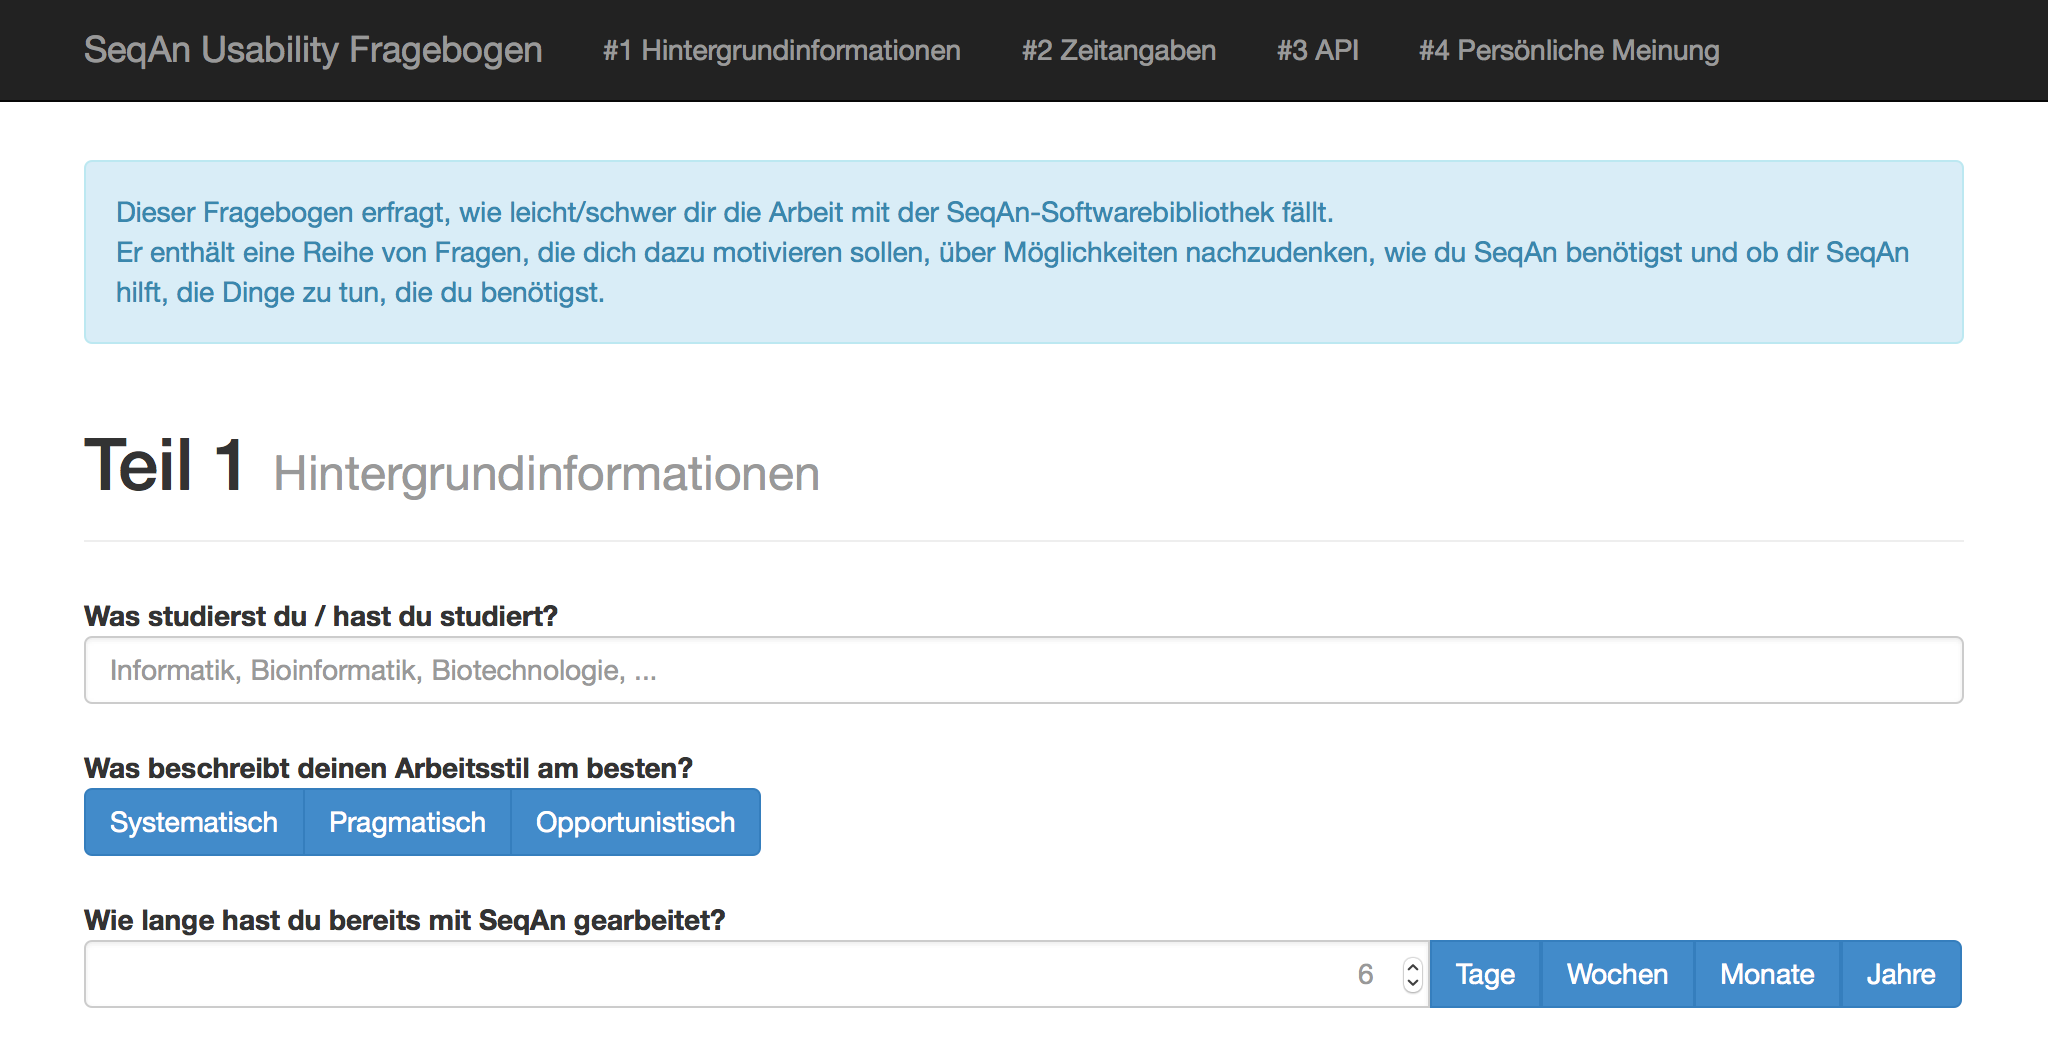
\includegraphics[width=1.0\linewidth]{Figures/cd-fragebogen-de-part.png}
    \caption{Ausschnitt aus dem deutschsprachigen Cognitive-Dimensions-Fragebogen}
    \label{fig:cd-fragebogen-de-part}
\end{figure}

Gemeinsam mit meinen Arbeitskollegen und den Autoren des Cognitive Dimension Frameworks Alan Blackwell und Thomas Green habe ich den Fragebogen mehrfach revisioniert. In einer Mail vom 21.03.2013 hat Alan Blackwell den Fragebogen abschließend mit ``looks nice'' beurteilt.


\subsubsection{Durchführung und Fazit}

Die Befragung mit Hilfe des Fragebogens fand im Rahmen des Workshops'13 statt.

Der von mir investierte Aufwand zeigt, dass es vollkommen unverhältnismäßig gewesen wäre, jedem Befragten diese Transfer-Leistung aufzubürden. An dieser Stelle kann man auch die Argumentation von \cite{Henning:2007kg,Ellis:2007kv} anwenden: Fragebögen werden von viel mehr Menschen ausgefüllt als entworfen. Es ist also ökonomisch absolut sinnvoll, die Instanziierung/Spezialisierung eines Fragebogens durch deren Autoren durchführen zu lassen.

\label{sec:cdf-usage-difficulties}
Insgesamt betrachtet, bleibt ein Cognitive-Dimensions-Fragebogen anspruchsvoll. Bei drei Probanden kam es bei jeweils einer Frage zu Missverständnissen\footnote{Beispiel: In einer Frage zu der CD \textit{Hard Mental Operations} wurde die Formulierung ``when combining things'' verwendet. Die Frage zielte auf die Verarbeitung verschiedener Informationen im Arbeitsgedächtnis abgezielt. Ein Proband jedoch bezog sie auf die Verknüpfung zwischen Funktion und dessen Dokumentationseintrag (siehe \url{apiua://survey/cd/2013-09-18T17:41:31.929+02:00/hardMentalOperations}).}. Eine Reihe von Fragen wurden von manchen Probanden nicht beantwortet. Die Begeisterung für den Fragebogen war geteilt. Ein Proband bezeichnete ihn als ``anstrengend''\citepurl{apiua://survey/cd/2013-09-18T17-45-54.88891500+0200/questionnaire}. Andere Probanden hingegen bewerteten den Fragebogen als ``Super''\citepurl{apiua://survey/cd/2013-09-18T17-46-05.89001200+0200/questionnaire} oder ``Klasse!''\citepurl{apiua://survey/cd/2013-09-18T17-50-13.42530400+0200/questionnaire}.

Die aufgefüllten Fragebögen wurden mit Hilfe der \gls{gtm} analysiert. Die Ergebnisse werden in den Abschnitten \ref{sec:phase4} und \ref{sec:Ergebnisse} vorgestellt.




\subsection{Programmierfortschritte-Erhebung}
\label{sec:programmierfortschritte}

Bei dieser Datenerhebungmethode handelt es sich um eine, die ich selbst entwickelt habe und in keiner mir bekannten Studie angewendet wurde. Sie besteht in der Erhebung von Daten, die den Entwicklungsprozess von Anwendungen, die von SeqAn-Anwendern entwickelt werden, nachvollziehbar machen sollen.


\subsubsection{Planung und Vorbereitung}

Um die Programmierfortschritte der verschiedenen SeqAn-Anwender dokumentieren zu können, benötigte ich die erstellten und veränderten Quellcode-Dateien, die bei der Programmentwicklung anfallen. Diese sollten bei jedem Versuch, den eigenen Programmcode zu kompilieren, erhoben werden, da davon auszugehen ist, dass dann ein irgendwie gearteter Arbeitsschritt abgeschlossen ist.

Um den Verständnisprozess des Anwenders besser verstehen zu können, interessierten mich auch die Zugriffe auf die Online-Dokumentation. Es war abzusehen, dass zwischen zwei Kompilierversuchen mehrere Minuten vergehen können. Die Zugriffe auf die Dokumentation sollten helfen, diese Lücken besser zu verstehen --- beispielsweise, ob ein SeqAn-Anwender gerade einen Dokumentationseintrag liest. Des Weiteren konnte ich so die Online-Dokumentation im Gebrauch durch den Anwender untersuchen. Dies zu können ist essentiell, weil die Dokumentation selbst Bestandteil der API im weiteren Sinne ist und eine wichtige Ressource zum Erlernen einer API darstellt \citep{Robillard:2009cs,Robillard:2010bh}.

Zu guter Letzt interessierten mich Daten zur Arbeitsumgebung, wie der verwendeten Entwicklungsumgebung.

Für die Datenerhebung selbst habe ich eine technische Lösung geplant und unter Verwendung einer Client-Server-Architektur implementiert.


\paragraph{Client}
\label{sec:apiua-client}

Die Datenerhebung auf den individuellen Arbeitsplätzen sollte so transparent laufen und einzurichten sein, wie möglich. 

SeqAn verwendet \textit{CMake}\footnote{\url{http://www.cmake.org}} als plattformübergreifendes Build-System. Als SeqAn-Anwender muss man bei der Installation, zunächst SeqAn herunterladen und dann, mit Hilfe von CMake, die notwendigen Projektdateien für die eigene Entwicklungsumgebung erstellen. Anschließend kann man mit SeqAn in der Entwicklungsumgebung seiner Wahl arbeiten.

Für die Datenerhebung habe ich die CMake-Dateien von SeqAn --- und damit den Build-Prozess --- so verändert, dass nach jedem Kompilierversuch ein Script ausgeführt wird, das Änderungen im SeqAn-Verzeichnis erkennt. Die betroffenen Dateien werden bei diesem Prozess in ein ZIP-Archiv gepackt und auf einen Datenerhebungsserver asynchon hochgeladen.

Der von mir entwickelte Datenerhebungsclient ist auf GitHub gehostet\footnote{\url{https://github.com/bkahlert/api-usability-analyzer-client-python}}.

\paragraph{Server}
\label{sec:apiua-server}

Die Server-Komponente dient der Sammlung der, von den Clients hochgeladenen Daten. Außerdem stellt er ein selbst entwickeltes JavaScript bereit, das in jede beliebige Webseite integriert werden kann und auf minutiöse Weise eine große Spannbreite an Ereignissen auf den instrumentierten Webseiten mitschneidet.

Die Server-Komponente habe ich in Form einer Java EE Web-Anwendung implementiert und auf GitHub bereitgestellt\footnote{\url{https://github.com/bkahlert/api-usability-analyzer-server-java-ee}}.

Das JavaScript zur Webseiten-Überwachung ist Bestandteil des Servers und verwendet ein interessantes Verfahren zur Umgehung der so genannten \textit{Same-Origin-Policy} (siehe \hyperref[subsec:same-origin-policy]{grauer Kasten}).

\begin{furtherreading}[frametitle={Website-Überwachung im Detail}]
\label{subsec:same-origin-policy}
Um eine Webseite (z.B. \texttt{client.com}) mit Hilfe des Datenerhebungsservers zu überwachen, muss zunächst eine JavaScript-Datei in die zu überwachende Seite eingebunden werden. Dies geschieht mit folgendem HTML-Code:
\begin{minted}[linenos=false, firstnumber=1, autogobble=false]{html}
<script src="https://srv.tld/SUAsrv/static/js/SUAclt.js"></script>
\end{minted}

Der kanonische Weg zur Übermittlung von Ereignissen, wie dem Laden oder Verlassen einer Seite, wäre die Absetzung einer Ajax-Anfrage\footnote{\url{http://www.w3.org/2007/06/mobile-ajax/}}. Dabei handelt es sich inhaltlich nicht um eine Anfrage sondern um eine Übermittlung von Daten (hier: Nutzeraktivitäten).

Ajax-Anfragen unterliegen jedoch der Same-Origin-Policy\footnote{\url{http://www.ibm.com/developerworks/web/library/wa-crossdomaincomm/index.html?ca=drs-\#N1019B}}, die den Zweck hat, Datendiebstahl und andere Angriffsformen zu verhindern. Die Übermittlung an einzelne Domains (hier: \texttt{srv.tld}) kann zwar erlaubt werden, wird allerdings nicht von älteren Browsern unterstützt\footnote{\url{https://developer.mozilla.org/en-US/docs/Web/HTTP/Access_control_CORS}}.

Um die Datenübermittlung auch bei älteren Browsern zu unterstützen, werden keine Ajax-Anfragen, sondern \textit{JSONP}-Anfragen\footnote{\url{http://bob.ippoli.to/archives/2005/12/05/remote-json-jsonp/}} abgeschickt. Technisch gesehen, wird dabei ein Script mit Hilfe des \texttt{<script>}-Tags in das \textit{Document Object Model} der überwachten Seite eingefügt, das ein Script lädt und dabei Parameter übergibt. Dabei dienen die belegten Parameter der Datenübermittlung. Das zurückgegebene Script enthält optional Rückgabedaten, die in diesem Fall aber irrelevant sind. Diese Art der Datenübermittlung unterliegt nicht der Same-Origin-Policy und erlaubt so die Übertragung der Nutzeraktivitäten.
\end{furtherreading}


\paragraph{Datenquelle: Arbeitsumgebung}

Für die Analyse der Programmierfortschritte kann es hilfreich sein, Daten zur Arbeitsumgebung des API-Anwenders zu kennen.
  
Dazu übermittelt der, weiter oben beschriebene Client bei der ersten Einrichtung der Entwicklungsumgebung Daten zum Betriebssystem und zur Entwicklungsumgebung an den Server. \lref{lst:apiua-data-demografisch} zeigt Inhalt und Struktur der übermittelten, JSON-formatierten Daten.

\begin{center}
\begin{minted}[linenos=false, firstnumber=1, autogobble=false]{json}
{
  "machine": {
    "machine": "x86_64",
    "processor": "i386",
    "architecture": "64bit"
  },
  "devenv": {
    "CMAKE_CXX_COMPILER": "/usr/bin/g++",
    "CMAKE_GENERATOR": "Xcode"
    },
  "os": {
    "platform": "Darwin-11.1.0-64bit"
    }
}
\end{minted}
\captionof{listing}{Beispiel: Daten zur Arbeitsumgebung}
\label{lst:apiua-data-demografisch}
\end{center}


\paragraph{Datenquelle: Quelldateien}

Bei jedem Kompilierversuch werden alle geänderten Dateien im SeqAn-Arbeitsverzeichnis vom Client in Form eines ZIP-Archivs an den Server übermittelt. Das Senden findet asynchron statt, um den Kompilierprozess nicht zu verlangsamen.

Das ZIP-Archiv erhält dabei einen Namen, der folgende Informationen enthält:
\begin{description}
  \item[ID] des Probanden. Diese ID identifiziert jeden Probanden eindeutig.
  \item[Hash-Wert] des SeqAn-Arbeitsverzeichnis-Pfades. Existieren mehrere SeqAn-Installationen auf einem Rechner, können diese so unterschieden werden.
  \item[Zeitpunkt] des Kompilierversuchs. Für den Zeitpunkt wird eine abgewandelte Form des, in der ISO 8601\footnote{\url{http://www.iso.org/iso/home/standards/iso8601.htm}} festgelegten Formats zur Darstellung von Datum und Zeit, verwendet. Diese Anpassung war notwendig, da beispielsweise der Doppelpunkt auf den meisten Dateisystemformaten nicht erlaubt ist.
\end{description}

Ein beispielhafter Name für ein übermitteltes ZIP-Archiv lautet: \texttt{6ndbc4zuiueuaiyv\_b9dc\_2013-04-09T10-31-07.379654+0200.diff.zip}.


\paragraph{Datenquelle: Onlinedokumentation}

Um die Verwendung einer Webseite durch einen Anwender nachvollziehen zu können, reicht es nicht, das Laden der entsprechenden Seite zu protokollieren.

Stattdessen müssen weitaus differenziertere Ereignisse protokolliert werden:
\begin{description}
  \item[READY] Die Seite wurde vollständig geladen.
  \item[UNLOAD] Die Seite wurde geschlossen.
  \item[FOCUS] Die Seite (bzw. der Browser-Tab) hat den Fokus erhalten.
  \item[BLUR] Die Seite (bzw. der Browser-Tab) hat den Fokus verloren.
  \item[RESIZE] Die Größe der Anzeigefläche wurde verändert. Üblicherweise passiert dies durch die Veränderung der Fenstergröße. Aber auch eingeblendete Browser-Menüs können dieses Ereignis provozieren.
  \item[SCROLL] Der Anwender hat innerhalb der Seite gescrollt.
  \item[TYPING] Der Anwender hat eine Text-Eingabe vorgenommen.
  \item[LINK] Der Anwender hat auf einen Link geklickt.
\end{description}

Bei jedem Ereignis werden, durch das vom Datenerhebungsserver ausgelieferte Script, eine Reihe von Daten asynchron übertragen: Zeitstempel, Ereignistyp, \acrshort{uri} der Seite, IP, Proxy-IP, Scrollposition und Größe der Anzeigefläche. Darüber hinaus werden Ereignis-abhängige Daten übermittelt, wie beim \textit{TYPING}-Ereignis die eigentliche Eingabe und der Name des Eingabefeldes.

Im \sref{sec:doclog} auf Seite \pageref{sec:doclog} stelle ich das Datenformat genauer vor. Dort befindet sich auch ein Auszug aus den so erfassten Daten (siehe \lref{lst:doclog-file}).



\paragraph{Identifikation und Datenschutz}
\label{sec:id}

Eben habe ich drei Datenquellen beschrieben, die in ihrer Gesamtheit die Programmierfortschritte eines Anwenders protokollieren. Allerdings stellt sich die Frage, wie die Datenquellen den Probanden zugeordnet werden können.

Die Identifikation eines Anwenders wird wie folgt realisiert:
\begin{itemize}
  \item Der Anwender muss die Datei \texttt{.APIUA} in seinem Benutzerverzeichnis anlegen. Damit weiß SeqAns Build-Prozess, dass eine Datenerhebung erlaubt ist. Darüber hinaus muss der Proband eine \textit{Einverständniserklärung zur Datenerhebung} (siehe \aref{app:declaration-of-consent}) unterschrieben haben, die ihn über den Umfang der Datenerhebung aufklärt.
  \item Bei der Einrichtung der SeqAn-Installation erfolgt durch den Anwender ein \textit{CMake}-Aufruf. Der von mir veränderte SeqAn-Build-Prozess prüft das Vorhandensein der \texttt{.APIUA}-Datei und aktiviert ggf. die Datenerhebung.
  \item Es wird eine zufällige 16-stellige alphanumerische ID erzeugt und in der Datei \texttt{.APIUA-ID} abgelegt --- ist sie bereits vorhanden, wird die darin enthaltene ID wiederverwendet.
  \item Der Standard-Browser wird geöffnet und eine spezielle Seite auf dem Datenerhebungsserver aufgerufen. Dabei wird die generierte ID an den Server übermittelt. Dem Anwender erscheint eine Seite, die sich für die Bereitschaft zur Datenübermittlung bedankt, die ID des Anwenders zeigt und das Verfahren zur Datenübermittlung erklärt (siehe \fref{fig:apiua-activation}).
  \item Die, auf dem Client erhobenen Arbeitsumgebungsdaten und Quelldateien enthalten in ihrem Dateinamen diese ID.
  \item Zur Identifikation des Browsers wird ein sogenannter \textit{Browser-Fingerprint} verwendet. Dabei wird ein Hash über diverse Datenpunkte (Browser, Betriebssystem, Zeitzone, etc.) berechnet.
  \item Durch den Aufruf der Bestätigungsseite erfährt der Server sowohl die übermittelte ID als auch den jeweils mit übermittelten Browser-Fingerprint. Dieses Tupel wird von dem Server gespeichert.
  \item Zukünftige Aufrufe von beobachteten Seiten übermitteln nun Nutzeraktivitäten an den Server. Mit Hilfe des Browser-Fingerprints, können diese Datenübermittlungen der ID des Anwenders zugeordnet werden.
  \item Der Browser-Fingerprint ist nicht dauerhaft stabil und kann sich, beispielsweise durch die Installation von Updates, verändern. Ich habe ein Verfahren entwickelt, dass überaus stabil ist und selbst das Löschen von Cookies überlebt. Mehr Details befinden sich im \hyperref[subsec:browser-fingerprint]{grauen Kasten}.
  \item Die im \sref{sec:feedback} beschriebenen Feedback-Zettel aus Phase 1, konnten von den Befragten ebenfalls mit ihrer ID versehen werden, um ein ganzheitliches Bild der Probanden zu erhalten (siehe \fref{fig:survey-id}).
\end{itemize}

\begin{figure}
  \centering
    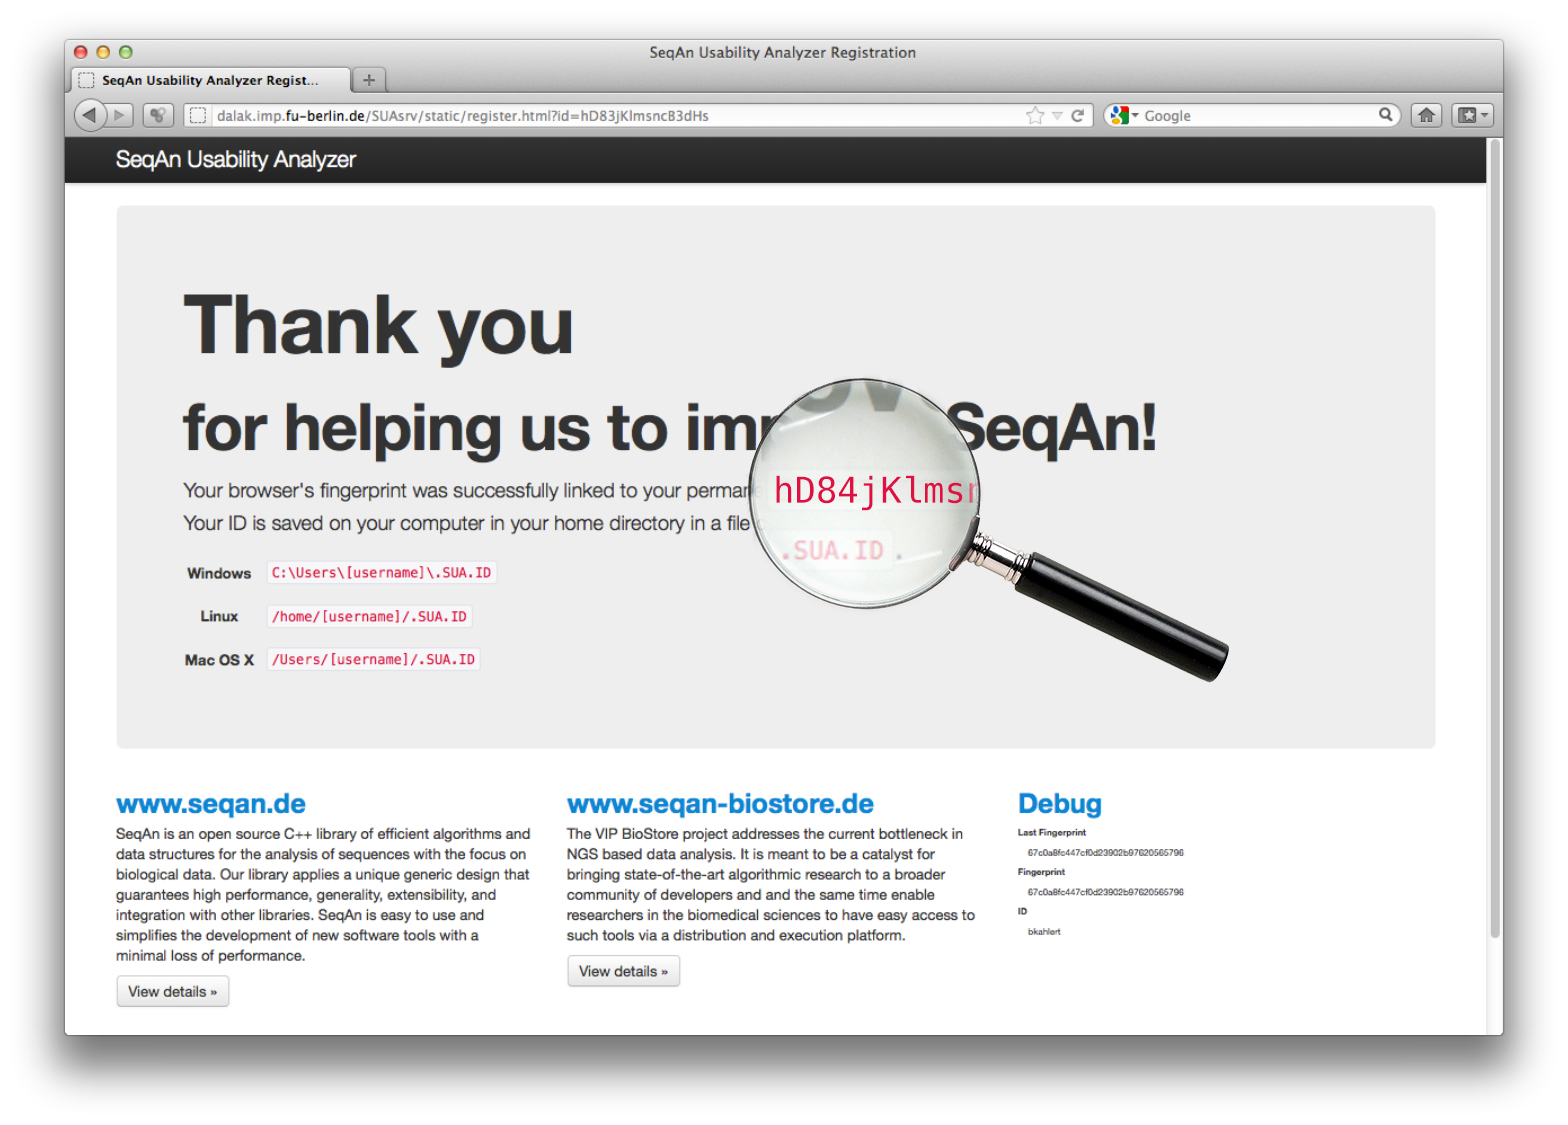
\includegraphics[width=0.75\linewidth]{Figures/apiua/activation.png}
  \caption{Bestätigung der Aktivierung der Datenerhebung}
  \label{fig:apiua-activation}
\end{figure}

Durch die ausschließliche Verwendung einer ID, setze ich das Prinzip der Pseudonymisierung um. Ein Rückschluss auf die Identität des Probanden ist so, stark erschwert. Ich hatte bei der Datenanalyse selbst mehrere Male das Bedürfnis, einen Probanden zu kontaktieren. Selbst mit dieser starken Motivation ist es mir nicht gelungen, die korrekte Person zu identifizieren.

Die Datenerhebung kann jederzeit vom Proband durch Löschen der Datei \texttt{.APIUA} eigenständig beendet werden.

\begin{furtherreading}[frametitle={Stabiles Browser-Fingerprinting}]
\label{subsec:browser-fingerprint}
Browser-Fingerprinting erfreut sich in der Online-Werbebranche großer Beliebtheit \citep{Bager:IDwRnNoQ} und verwendet diverse Merkmale, die der Browser (a) in seiner HTTP-Anfrage mitschickt oder (b) sich mit JavaScript auslesen lassen. Durch installierte Plugins, wie Flash oder Java, steigt der verwendbare Merkmalumfang weiter an. Ein Großteil, der weltweit eingesetzten Browser-Installationen, ist durch diese Merkmale eindeutig identifizierbar\footnote{\url{http://m.heise.de/newsticker/meldung/Fingerprinting-Viele-Browser-sind-ohne-Cookies-identifizierbar-1982976.html}\\\url{https://panopticlick.eff.org/browser-uniqueness.pdf}}.

Je mehr Merkmale für den Browser-Fingerprint verwendet werden, desto wahrscheinlicher ist eine eindeutige Erkennbarkeit. Allerdings steigt so auch die Wahrscheinlichkeit einer Veränderung des Browser-Fingerprints.

Um einen Browser dauerhaft zu identifizieren, benötigt man einen Mechanismus, der es einem erlaubt, den alten und den neuen Browser-Fingerprint in Erfahrung zu bringen.

Dazu muss zunächst der alte Browser-Fingerprint im Browser --- z.B. in Form eines Cookies --- gespeichert werden. Cookies (und alle anderen lokalen Speicherformen) setzen die Same-Origin-Policy um. Das heißt, dass ein, auf einer beliebigen  Seite \textit{example.com} eingefügtes Datenerhebungsscript von \textit{server.com}, nicht die Cookies der jeweils anderen Domain auslesen kann. Das Datenerhebungsscript arbeitet im Kontext von \textit{example.com}, muss aber Cookies im Kontext von \textit{server.com} ablegen, damit es Anwender, über mehrere Domains hinweg, verfolgen kann.

Um das zu erreichen, erzeugt mein Datenerhebungsscript im \textit{Document Object Model} von \textit{example.com} ein unsichtbares \textit{IFrame} und lädt darin eine speziell präparierte HTML-Seite von \textit{server.com}. Diese spezielle Seite verfügt selbst über ein JavaScript, das nun Cookies im Kontext von \textit{server.com} anlegen und so den alten Fingerprint im Browser speichern kann. Verändert sich nun der Browser-Fingerprint, kann \textit{server.com} den alten Fingerprint aus dem Cookie auslesen und die, unter dem alten Fingerprint gespeicherten Daten auf den neuen Fingerprint umschreiben.

Tatsächlich ist das Problem noch ein ganzes Stück komplexer. Für die Kommunikation zwischen der Seite und dem IFrame übergebe ich Daten über das \texttt{window.name}-Objekt\footnote{\url{https://bugzilla.mozilla.org/show_bug.cgi?id=444222}} und für die Datenablage verwende ich alle erdenklichen Speichermöglichkeiten (\textit{local storage}, \textit{flash cookies}, etc.), wie es das \textit{evercookie} \citep{Kamkar:FIOYXZjo} vormacht. Löscht der Anwender nicht sämtliche Speicherorte auf einmal, stellt \textit{evercookie} sicher, dass die gespeicherten Informationen wieder mit allen Speicherorten synchronisiert werden. Der Anwender kann die, in seinem Browser gespeicherten Informationen praktisch nicht löschen\footnote{\url{http://www.heise.de/newsticker/meldung/User-Tracking-Werbefirmen-setzen-bereits-haeufig-nicht-loeschbare-Cookie-Nachfolger-ein-2264381.html?wt_mc=rss.ho.beitrag.atom}}.
\end{furtherreading}

\begin{figure}
  \centering
    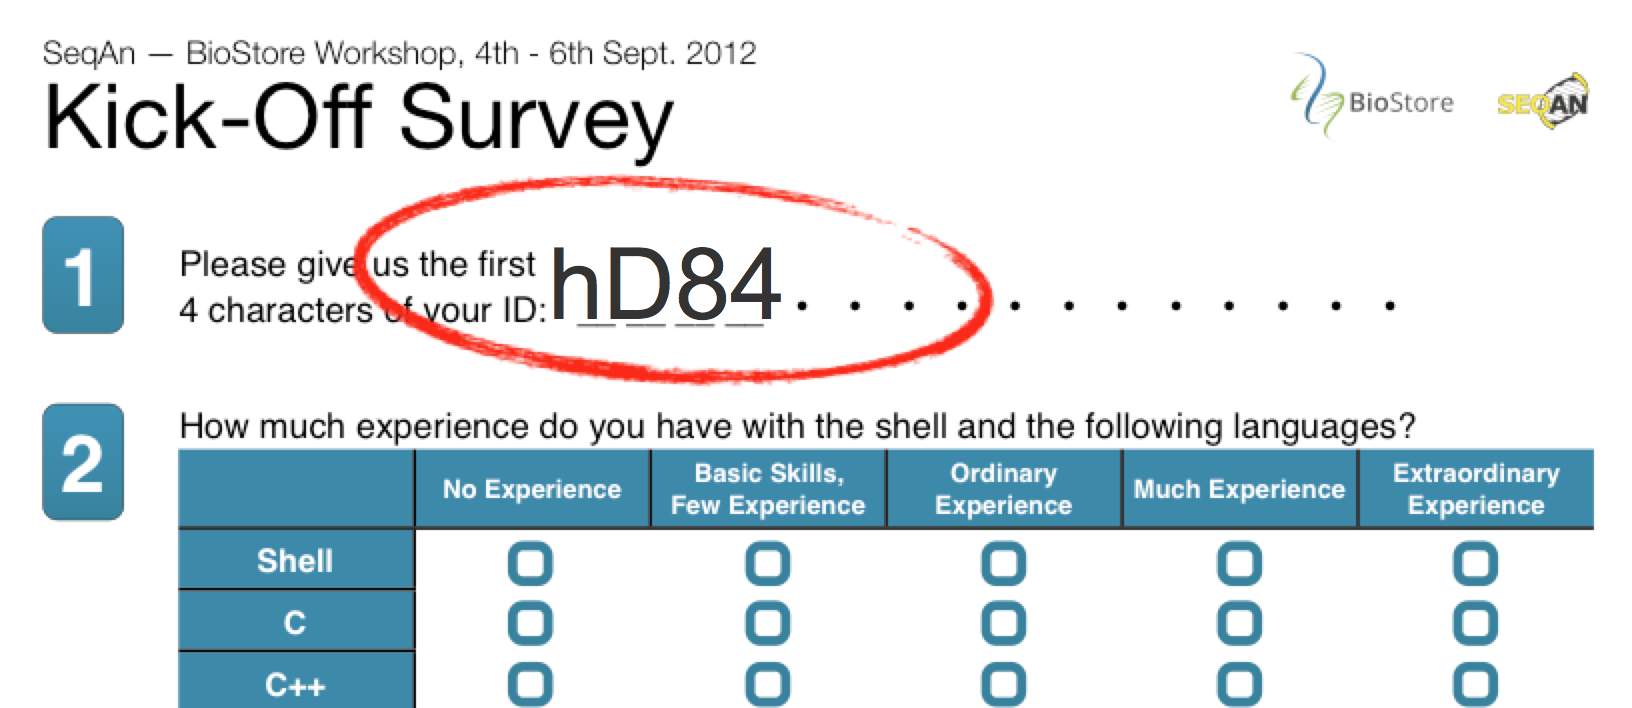
\includegraphics[width=0.75\linewidth]{Figures/survey-id.png}
  \caption{Eintragung der ID im Feedback-Zettel}
  \label{fig:survey-id}
\end{figure}
  
  
  
\subsubsection{Durchführung und Fazit}
\label{sec:phase2-programmierfortschritte-durchfuhrung}

Aktivitäten wurden auf den Webseiten für die Online-Dokumentation und für die Tutorials protokolliert.

Die Aufzeichnung der Programmierfortschritte fand bei allen Workshops ('11, '12 und '13), sowie bei zwei von drei PMSB-Praktika ('12, '13) statt. Des Weiteren konnte ich einen Langzeitprobanden gewinnen. Dieser Datensatz umfasst mehr als 1.200 Entwicklungsschritte. Insgesamt liegen Datensätze zu über 50 Probanden vor.

Zur Analyse der Datensätze kam die \gls{gtm} zum Einsatz. Wegen des hohen Aufwand zur Analyse dieser Daten, wurden nur wenige Datensätze betrachtet. Die Ergebnisse werden in den Abschnitten \ref{sec:phase4} und \ref{sec:Ergebnisse} vorgestellt.

Die hier präsentierte Datenerhebungsmethode unterscheidet sich von den, üblicherweise gebräuchlichen Videoaufzeichnungen \citep[vgl.][]{clarke:2006,LaToza:2007fj,Grill:2012jm,Piccioni:2013uq}. Es arbeitet Plattform- und Entwicklungsumgebung-übergreifend, erfordert keine Anpassungen am Arbeitsplatz der Probanden und eignet sich für Langzeitstudien, was die Beobachtung von Usability-Problemen erlaubt, die nicht in einem einzelnen Messpunkt zu finden sind oder erst nach einem längeren Gebrauch einer API auftreten. Technisch gesehen, könnte dieses Verfahren sogar vollkommen transparent, automatisiert und ohne jedes anwenderseitige Zutun eingesetzt werden.

Vergleichbare, manuell einzurichtende Datenerhebungen haben \cite{LaToza:2007fj,Layman:2008:MIU:1370114.1370133} implementiert. Dabei wurde jedoch \gls{eclipse} instrumentalisiert, was andere Entwicklungsumgebungen ausschließt. Der Vorteil besteht allerdings darin, dass mit einem \gls{eclipse}-Plugin auch feingranularere Ereignisse erfasst werden können. Browserzugriffe werden hingegen nicht von deren Datenerhebungen erfasst.

Die Datenerhebungsmethode wurde im Verlauf dieser Studie mehrfach verbessert. Während der ersten Datenerfassung wurden Schwächen deutlich, die beseitigt werden mussten. Diese Behebungen waren teilweise sehr aufwändig, da die bereits erhobenen Daten immer wieder auf aktualisierte Datenformate umgestellt werden mussten. Die folgende Auflistung nennt die wichtigsten Verbesserungen: \label{sec:datenerhebung-probleme}
\begin{itemize}
  \item Manche Anwender verwendeten mehrere SeqAn-Installationen oder mehrere Entwicklungsumgebungen. Die entsprechende Unterstützung musste implementiert werden, um unterschiedliche Programmentwicklungsverläufe unterscheiden zu können.
  \item Bei den ersten Datenerhebungen wurde die Zeitzone nicht mit erfasst. Dies führte bei einem Teilnehmer zu Problemen, da der Server eine andere Zeitzone verwendete und damit die verschiedenen Datenquellen zeitlich verschoben waren. Die Datenerhebung wurde um eine entsprechende Zeitzonen-Unterstützung ergänzt.
  \item Ursprünglich wurden nicht die geänderten Dateien, sondern nur das Dateien-Diff\footnote{\url{https://www.gnu.org/software/diffutils/}} übertragen. Bei fehlerhaften Datenerhebungen führte das dazu, dass die späteren Dateistände nur noch händisch oder gar nicht mehr rekonstruiert werden konnten.
  \item Fehler bei der Datenerhebung wurden nicht protokolliert. Eine entsprechende Protokollierung wurde implementiert. Auftretende Fehler werden nun an eine zuvor hinterlegte E-Mail-Adresse weitergeleitet.
  \item Die große Bandbreite an möglichen Konfigurationen auf Probandenseite, machte automatisierte Tests notwendig. Dieses Tests umfassen alle hier vorgestellten Datenquellen. Dabei kam das Code-Coverage-Tool \textit{EclEmma}\footnote{\url{http://www.eclemma.org}} zum Einsatz. Für das Testen der verschiedenen Browser verwendete ich \textit{Selenium}\footnote{\url{http://www.seleniumhq.org}}.
  \item Die Unterstützung von SSL-basierten Webseiten wurde implementiert, weil einige Webseiten sowohl über HTTP, als auch über HTTPS verfügbar sind.
  \item Die Datenerhebung wurde --- wo es möglich war --- parallelisiert und asynchron implementiert.
  \item Die Webseiten-Ereignisse \textit{FOCUS} und \textit{BLUR} wurden hinzugefügt, um besser nachvollziehen zu können, ob und welche Webseite bzw. Browser-Tab gerade gelesen wird.
\end{itemize}

Ein Problem konnte nicht gelöst werden: Der Erfolg oder Misserfolg von Kompilierversuchen konnte nicht protokolliert werden. Dies ist ohne größeren Aufwand nicht Plattform- und Entwicklungsumgebung-übergreifend möglich. Eine Option besteht darin, die verschiedenen Dateistände nachträglich zu kompilieren. Eine zuverlässige Rekonstruktion würde jedoch die Bereitstellung der entsprechenden Arbeitsumgebungskonfigurationen erfordern, was seine eigenen Probleme mit sich bringt.



\subsection{Zusammenfassung}
\label{sec:phase2-fazit}

In diesem Abschnitt habe ich ein umfassendes Datenerhebungsverfahren vorgestellt.

Durch die Erfassung von Programmierfortschritten erlaubt dieses Datenerhebungsverfahren, im Gegensatz zu fast allen mir bekannten Arbeiten, Langzeitstudien durchzuführen. Die erhobenen Daten werden nicht durch die Erzwingung der Arbeit an einem, für eine Datenerhebung vorbereiteten Arbeitsplatz verfälscht. Darüber hinaus wird die Datenerhebung durch das einfache Anlegen bzw. Löschen einer Datei aktiviert bzw. deaktiviert und der Anwender nicht abgelenkt.

Die objektiven Daten werden durch subjektive Daten ideal ergänzt, da sie teilweise verschiedenartige Usability-Probleme beherbergen. Subjektive Daten können außerdem Orientierung für die Analyse der objektiven Daten geben. Sie werden mit Hilfe einer Gruppendiskussion und dem hier vorgestellten Cognitive-Dimensions-Fragebogen erhoben.

Das Datenerhebungsverfahren wird meinen speziellen Anforderungen gerecht. Durch die nicht beeinflussbaren Datenerhebungsmöglichkeiten, war eine besonders hohe Reichhaltigkeit vonnöten, denn weitere Datenerhebungen im Sinne des \textit{theoretischen Samplings} waren nicht ohne weiteres möglich. Dieser Ansatz ist tolerabel, denn einerseits umfassen die Daten bereits verschiedene Datenquellen, was dem Triangulierungsgütekriterium entgegenkommt und andererseits erlaubt die Reichhaltigkeit der Daten weitere Analysen unter einem anderen Betrachtungswinkel. 

Die Teilnehmer der Workshops und PMSB-Praktika repräsentieren hinreichend die SeqAn-Anwendergruppe.

Die verschiedenen Datenerhebungen wurden bei den folgenden Veranstaltungen wie folgt durchgeführt:
\begin{description}
  \item[Workshops] \hfill
  \begin{description}
    \item[Workshop'11] \textit{13.-15.09.2011}
    \begin{description}
%      \item[Fragebögen] von xx Teilnehmer
      \item[Programmierfortschritte] von 13 Teilnehmern
    \end{description}
    
    \item[Workshop'12] \textit{04.-06.09.2012}
    \begin{description}
%      \item[Interviews] mit keinem der Teilnehmer, da es wegen der hohen Veranstaltungsdichte keinen Raum dazu gab
      \item[Gruppendiskussion] von rund 20 Teilnehmern
      \item[Programmierfortschritte] von 14 Teilnehmern
    \end{description}
     
    \item[Workshop'13] \textit{17.-19.09.2013}
    \begin{description}
      \item[Cognitive-Dimensions-Fragebogen] von 10 Teilnehmer
      \item[Programmierfortschritte] von 16 Teilnehmern
    \end{description}
  \end{description}
  
  \item[PMSB] \hfill
    \begin{description}
    \item[PMSB'12] \textit{05.2012}
    \begin{description}
%      \item[Interviews] mit 4 Teilnehmer
      \item[Programmierfortschritte] von 6 Teilnehmern
    \end{description}
    
    \item[PMSB'13] \textit{04.2013}
    \begin{description}
      \item[Fragebögen] von xx Teilnehmer
      \item[Programmierfortschritte] von 10 Teilnehmern
    \end{description}
    
    \item[PMSB'14] \textit{04.2014}
    \begin{description}
      \item[Programmierfortschritte] nicht erhoben
    \end{description}
  \end{description}
  
  \item[Langzeitprobanden] \hfill
  \begin{description}
    \item[Programmierfortschritte] von einem Teilnehmer %Langzeitproband David Meyer gewonnen (03.07.2012, brbym28nz827lxic) über 1200 Revisionen
  \end{description}
\end{description}

\bigskip

Da nun die Daten erhoben werden konnten, dürfte der Analyse Selbiger mit Hilfe der \gls{gtm} nichts im Weg stehen. Allerdings unterstützte kein gängiges Datenanalysewerkzeug die qualitative Analyse dieser hoch-strukturierten Daten. Aus diesem Grund musste ich selbst ein Werkzeug entwickeln, das ich im folgenden Abschnitt vorstelle.

In Phase 4 (\sref{sec:phase4}) werde ich schließlich die eigentliche Forschung mit Hilfe der \gls{gtm} und meinem Datenanalysewerkzeug besprechen.